% Adriano Bassignana nov 2017
% Program for creating a linear index useful for the construction of a compass on a conical support
% The program can be modified and adapted for the construction of other types of numeric indexes.
% The font used is OCR-B which allows to have alphabetic and numeric symbols very similar
% to those used in analogue flight gauges in the 50s and 80s
% You must have installed OCR-B in OTF format that has a GPL-2 and later compatible license.
% The font is present in the texlive-fonts-extra package
% 
% Explanation:
%
% \documentclass{standalone} is particular class that non have a size, but the size is define from
% the document itself
\documentclass[tikz,margin=0pt]{standalone}
% \usepackage{tikz} is the package that contain the graphics command as \draw etc ...
% The package is describe in this document: https://www.sharelatex.com/learn/TikZ_package
\usepackage{tikz}
% If the graduate dials is for analogical gauges period 50-70 years, this font is ok
% OCR is open-source package deposited in the CTAN repository: https://www.ctan.org/pkg/ocr-b
% Opentype can be used on Linux and Mac machines
% (I do not know if it's possible in Windows, but I think of it),
% you can always download it from the CTAN site at this address:
% https://www.ctan.org/tex-archive/fonts/ocr-b-outline
\usepackage{ocr}
% Defines the font size to use, the first number defines the font size,
% the second number the dimensional family from which the font is taken.
% It can be assumed that there are differences between a dimensional family 10 and a 12 dimensional font.
\tikzset{font={\fontsize{18pt}{10}\selectfont}}
\begin{document}
% The link OCR package documentation is this: http://ctan.mirror.garr.it/mirrors/CTAN/macros/latex/contrib/ocr-latex/ocr.pdf
% \ocrfamily - Normal font family
% \ocrnegfamily - Family negative fonts
{\ocrfamily
    % Xscale defines the scale of the drawing with respect to the document we write.
    % It is imperative to make it compatible for the size of the graduated dial that we are designing.
    % Its determination requires a number of tests to optimize the font dimension with the units of measurement.
    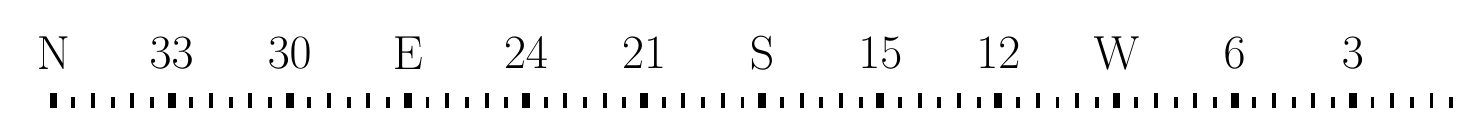
\begin{tikzpicture}[xscale=0.05]
      %5° Rays
      \foreach \a in {0, 5,...,355}
	\draw[line width=0.5mm] (\a,0) -- (\a,1.5mm);
      %10° Rays
      \foreach \a in {0, 10,...,350}
	\draw[line width=0.5mm] (\a,0) -- (\a,2.0mm);
      %30° Rays
      \foreach \a in {0, 30,...,345}
	\draw[line width=1mm] (\a,0) -- (\a,2.0mm); 
      %labels  
      \draw (30,0.7) node {33};
      \draw (60,0.7) node {30};
      \draw (120,0.7) node {24};
      \draw (150,0.7) node {21};
      \draw (210,0.7) node {15};
      \draw (240,0.7) node {12};
      \draw (300,0.7) node {6};
      \draw (330,0.7) node {3};
      \draw (0,0.7) node {N};
      \draw (90,0.7) node {E};
      \draw (180,0.7) node {S};
      \draw (270,0.7) node {W};
    \end{tikzpicture}
}
\end{document}